% --------------------------------------------------------------
% This is all preamble stuff that you don't have to worry about.
% Head down to where it says "Start here"
% --------------------------------------------------------------
 
\documentclass[12pt]{article}
 
\usepackage[margin=1in]{geometry} 
\usepackage{bm} % bold in mathmode \bm
\usepackage{amsmath,amsthm,amssymb,mathtools}
\usepackage{dsfont} % for indicator function \mathds 1
\usepackage{tikz,pgf,pgfplots}
\usepackage{enumerate} 
\usepackage[multiple]{footmisc} % for an adjascent footnote
\usepackage{graphicx,float} % figures

\newtheorem{definition}{Definition}
\let\olddefinition\definition
\renewcommand{\definition}{\olddefinition\normalfont}
\newtheorem{lemma}{Lemma}
\let\oldlemma\lemma
\renewcommand{\lemma}{\oldlemma\normalfont}
\newtheorem{proposition}{Proposition}
\let\oldproposition\proposition
\renewcommand{\proposition}{\oldproposition\normalfont}
\newtheorem{corollary}{Corollary}
\let\oldcorollary\corollary
\renewcommand{\corollary}{\oldcorollary\normalfont}
\newtheorem{theorem}{Theorem}
\let\oldtheorem\theorem
\renewcommand{\theorem}{\oldtheorem\normalfont}

\newcommand\norm[1]{\left\lVert#1\right\rVert} % \norm command 

%%% PLOTTING PARAMETERS
\tikzstyle{bag} = [text width=7em, text centered] %binomial tree node width
\tikzstyle{end} = []
%%%

%% set noindent by default and define indent to be the standard indent length
\newlength\tindent
\setlength{\tindent}{\parindent}
\setlength{\parindent}{0pt}
\renewcommand{\indent}{\hspace*{\tindent}}

\newcommand*{\vv}[1]{\vec{\mkern0mu#1}} % \vec command

%% DAVIDS MACRO KIT %%
\newcommand{\R}{\mathbb R}
\newcommand{\N}{\mathbb N}
\newcommand{\Z}{\mathbb Z}
\renewcommand{\P}{\mathbb P}
\newcommand{\Q}{\mathbb Q}
\newcommand{\E}{\mathbb E}
\newcommand{\var}{\mathrm{Var}}
\newcommand{\indist}{\,{\buildrel \mathcal D \over \sim}\,}

\newcommand{\bigtau}{\text{{\large $\bm \tau$}}}

\begin{document}
 
% --------------------------------------------------------------
%                         Start here
% --------------------------------------------------------------
 
\title{Mathematical \& Computational Finance I\\Lecture Notes}
\author{Probability Theory on Coin Toss Space}
\date{January 28 2016 \\ Last update: \today{}}
\maketitle

% SECTION: 
\section{Markov Processes}

\indent We must determine the relevant variables when calculating derivative security prices and design appropriate algorithms that may be efficiently implemented.

\begin{definition} On a finite probability space $(\Omega, \P)$, such as the binomial model, let the process $\{X_n\}^N_{n = 0}$ be adapted. If for every $n \in \{0,1,..., N - 1\}$ and for every function $f(x)$ there exists some function $g(x)$, which may depend on $n$ and $f$, such that
\begin{equation*}
	\E_n\left[ f(X_{n + 1}) \right] = g(X_n)
\end{equation*}

then $\{X_n\}^N_{n = 0}$ is a \underline{Markov process}. That is, the value at some time $n + 1$ given all the information up to time $n$ is only a function of the value at time $n$ and not the path for which the random variable takes.
\end{definition}

We should now take a moment to note that the martingale property
\begin{equation*}
	\E_n \left[X_{n + 1} \right] = X_n
\end{equation*}

is a special case of the Markov property with $f(x) = x \implies g(x) = x$. We also note that $\E_n \left[ f(X_{n + 1}) \right](\omega_1\cdots\omega_n)$ is a random variable depending on the first $n$ coin tosses. The Markov property given by the above equation gives us that this dependence is characterized by the value given by $X_n(\omega_1\cdots\omega_n)$. \\

For derivative security pricing the Markov property tells us that
\begin{enumerate}[]
	\item {\bf IF} the derivative security payoff at time $N$ is random only though its dependence on the value of $X_N$
	\item {\bf THEN} there exists a version of the pricing algorithm in which we do not need to store path information.
\end{enumerate}

\indent The task is to find the corresponding function $g$ in order to verify the Markov property of some function of a random variable. \\

\underline{Example}: In the binomial asset pricing model we may write the stock price process\footnote{The binomial model is an adapted process by its construction.} as
\begin{equation*}
	S_{n + 1}(\omega_1\cdots\omega_n\omega_{n + 1}) = 
	\begin{cases}
		uS_n(\omega_1\cdots\omega_n) & \text{if } \omega_{n + 1} = H \\
		dS_n(\omega_1\cdots\omega_n) & \text{if } \omega_{n + 1} = T
	\end{cases}
\end{equation*}

Therefore, for an arbitrary function $f(x)$ and arbitrary probabilities $p$ and $q = 1 - p$,
\begin{equation*}
	\E_n \left[f(S_{n + 1}) \right](\omega_1\cdots\omega_n) = pf(uS_n(\omega_1\cdots\omega_n)) + qf(dS_n(\omega_1\cdots\omega_n)) =: g(S_n)
\end{equation*}

so that
\begin{equation*}
	\E_n \left[ f(S_{n + 1}) \right] = g(S_n)
\end{equation*}

where
\begin{equation*}
	g(x) = pf(ux) + qf(dx)
\end{equation*}

{\bf Therefore, the stock price process is Markovian}. \\

\indent We have just shown that stock price is Markovian with respect to both the real world measure $\P$ and the risk neutral measure $\tilde{\P}$. In order to determine the price $V_n$ at time $N$ of a derivative security whose payoff at time $N$ is a function $\nu_N$ of the stock price at time $N$
\begin{equation*}
	V_N = \nu_N(S_N)
\end{equation*}

the risk neutral pricing formula gives us
\begin{equation*}
	V_n = \frac{1}{1 + r} \tilde{\E}_n[V_{n + 1}] \quad n = 0, 1,..., N - 1
\end{equation*}

\indent However, we wish to find $\nu_N$ such that $V_N = \nu_N(S_N)$. We know that the stock price process is Markovian, so
\begin{equation*}
	V_{N - 1} = \frac{1}{1 + r} \tilde{\E}_{N - 1} \left[ \nu_N(S_N) \right] = \nu_{N - 1}(S_{N - 1})
\end{equation*}

for some function $\nu_{N - 1}$. Similarly,
\begin{equation*}
	V_{N - 2} = \frac{1}{1 + r} \tilde{\E}_{N - 2} \left[ \nu_{N - 1}(S_{N - 1}) \right] = \nu_{N - 2}(S_{N - 2})
\end{equation*}

\indent Continuing with this process we find that in general $V_n = \nu_n(S_n)$ for some function $\nu_n$. Then we can compute from the risk neutral pricing formula
\begin{equation*}
	\nu_n(s) = \frac{1}{1 + r} \left[ \tilde{p} \nu_{n + 1}(us) + \tilde{q}\nu_{n + 1}(ds) \right] \quad n = 0, 1, ..., N - 2, N - 1
\end{equation*}

\indent This algorithm works for any derivative security whose payoff at time $N$ is only a function of $S_N$, that is, any derivative whose payoff is Markovian/path independent. This algorithm works in the binomial model for any derivative security where the time $N$ payoff is a function only of the time $N$ stock price. In particular, we use the same algorithm for pricing put and call options -- the only difference being the function $\nu_N(s)$: We have $\nu_N(s) = (K - s)^+$ and $\nu_N(s) = (s - K)^+$ for puts and calls, respectively.

\subsection{Independence Lemma}

\begin{lemma} {\bf Independence Lemma 1.0:} In the $N$-period binomial asset pricing model let $n \in \{0, 1, ..., N\}$. Suppose that the random variables $X^1, ..., X^K$ depend only on coin tosses $1$ through $n$ and $Y^1,..., Y^L$ depend only on the following coin tosses $n + 1$ through $N$. \\

Let $f(x^1,...x^K,y^1,...y^L)$ be a function of $K + L$ variables. Then
\begin{equation*}
	\E_n \left[ f(X^1,...X^K,Y^1,...,Y^L) \right] = g(X^1,...X^K)
\end{equation*}

where
\begin{equation*}
	g(x^1,...,x^K) = \E\left[ f(x^1,...x^K,Y^1,...Y^K) \right]
\end{equation*}

\indent The Independence Lemma takes its name from the fact that the random variables $Y^1,...Y^K$ are \underline{independent} of the first $n$ coin tosses.

\begin{proof} %If we think of this as two (potentially vector valued) random variables $X$ and $Y$ then
%\begin{equation*}
%	\E_n \left[ f(X,Y) \right] = \int \int p_n(x,y)\,dx\,dy
%\end{equation*}

%where $p_n$ is the joint probability mass function of $X$ and $Y$.

Fix the first $n$ arbitrary coin tosses. By definition we have
\begin{align*}
	\E_n [f(X, Y)](\omega_1\cdots\omega_n) &= \sum_{\omega_{n + 1}\cdots\omega_N} p^{\#H(\omega_{n + 1}\cdots\omega_N)} q^{\#T(\omega_{n + 1}\cdots\omega_N)} f(X(\omega_1\cdots\omega_N), Y(\omega_1\cdots\omega_N)) \\
	&\equiv \sum_{\omega_{n + 1}\cdots\omega_N} p^{\#H} q^{\#T} f(X(\omega_1\cdots\omega_N),Y(\omega_1\cdots\omega_N)) \\
	&= \sum_{\omega_{n + 1}\cdots\omega_N} p^{\#H} q^{\#T} f(X(\omega_1\cdots\omega_n),Y(\omega_{n + 1}\cdots\omega_N))
\end{align*}

since $X$ is only a function of coin tosses 1 through to $n$ and $Y$ only a function of tosses $n + 1$ through to $N$. Now, note 
\begin{align*}
	g(x) &= \E[f(x,Y)] \\
	&= \sum_{\omega_{n + 1}\cdots\omega_N} p^{\#H}q^{\#T} f(x, Y(\omega_{n + 1}\cdots\omega_N))
\end{align*}

Therefore, equating both parts together, we find
\begin{equation*}
	g(X(\omega_1\cdots\omega_n)) = \E_n \left[ f(X, Y) \right](\omega_1\cdots\omega_n)
\end{equation*}

hence
\begin{equation*}
	\E_n[f(X,Y)] = g(X) = \E[f(X,Y)]
\end{equation*}

for $X$ dependent on the first $n$ coin tosses and $Y$ dependent only on the next $n + 1$ to $N$ coin tosses, as desired.
\end{proof}
\end{lemma}

If we think about
\begin{enumerate}
	\item Vector valued random variables $X = (X^1,...,X^K)$ and $Y = (Y^1,...,Y^L)$.
	\item $X$ being {\bf measureable} with respect to the information avaiable at time $n$ (which we denote by the sub-$\sigma$-algebra $\mathcal G_n$.
	\item $Y$ being {\bf independent} of the information available at time $n$ 
\end{enumerate}

then we can restate the lemma as

\begin{lemma} {\bf Independence Lemma 2.0:} If the random vector $X$ is measurable with respect to $\mathcal G_n$ and the random vector $Y$ is independent of $\mathcal G_n$ then
\begin{equation*}
	\E \left[ f ( X,Y ) \Big| \mathcal G_n \right] = g(X)
\end{equation*}

where 
\begin{equation*}
	g(x) = \E \left[ f(x, Y ) \right]
\end{equation*}

If $f$ was linear then this would be equivalent to ``taking our what is known''.
\end{lemma}

\underline{Example}: Consider the vector valued random variables $X$ and $Y$ such that $X$ is dependent only on coin tosses 1 through $n$ and $Y$ is dependent only on coin tosses $n + 1$ through $N$. If we had $f(x,y) = xy$ such that $\E_n[XY]$ then we may rewrite this as
\begin{equation*}
	\E_n[XY] = X\E_n[Y]
\end{equation*}

and since $Y$ is independent on the first $n$ coin tosses
\begin{align*}
	\E_n[XY] &= X\E_n[Y] \\
	&= X\E[Y]
\end{align*}

\indent Often we use the Independence Lemma to price something that is Markovian, but this begs the question of how to prove that some process is in fact Markovian? Going back to the definition we require that the process
\begin{enumerate}[(i)]
	\item be adapted
	\item the Markov property holds, that is, $\E_n[f(X_{n + 1})] = g(X_n)$ for all functions $f$
\end{enumerate}

\underline{Example}: (Non-Markovian process) Consider the maximum process. We think of this as dependent on the path the process takes. Let $S_0 = 4, u = 2, d = \frac{1}{2}, M_n = \max_{0 \leq k \leq n} \left\{S_k\right\}, p = \frac{2}{3}, q = \frac{1}{3}$. We have the binomial trees

\begin{figure}[H]
\begin{tikzpicture}[sloped]
  \node (a) at ( 0,0) [bag] {$S_0 = 4$};
  \node (b) at ( 2,-1.5) [bag] {$S_1(T) = 2$};
  \node (c) at ( 2,1.5) [bag] {$S_1(H) = 8$};
  \node (d) at ( 6,-3) [bag] {$S_2(TT) = 1$};
  \node (e) at ( 6,0) [bag] {$S_2(HT) = S_1(TH) = 4$};
  \node (f) at ( 6,3) [bag] {$S_2(HH) = 16$};
  \node (g) at ( 12,-4.5) [bag] {$S_3(TTT) = \frac{1}{2}$};
  \node (h) at ( 12,-1.5) [bag] {$S_3(HTT) = S_3(THT) = S_3(TTH) = 2$};
  \node (i) at ( 12,1.5) [bag] {$S_3(HHT) = S_3(HTH) = S_3(THH) = 8$};
  \node (j) at ( 12,4.5) [bag] {$S_3(HHH) = 16$};
  \draw [->] (a) to node [below] {} (b);
  \draw [->] (a) to node [above] {} (c);
  \draw [->] (c) to node [below] {} (f);
  \draw [->] (c) to node [above] {} (e);
  \draw [->] (b) to node [below] {} (e);
  \draw [->] (b) to node [above] {} (d);
  \draw [->] (d) to node [below] {} (g);
  \draw [->] (d) to node [above] {} (h);
  \draw [->] (e) to node [below] {} (h);
  \draw [->] (e) to node [above] {} (i);
  \draw [->] (f) to node [below] {} (i);
  \draw [->] (f) to node [above] {} (j);
\end{tikzpicture}
\caption{Asset price process tree}
\end{figure}

\begin{figure}[H]
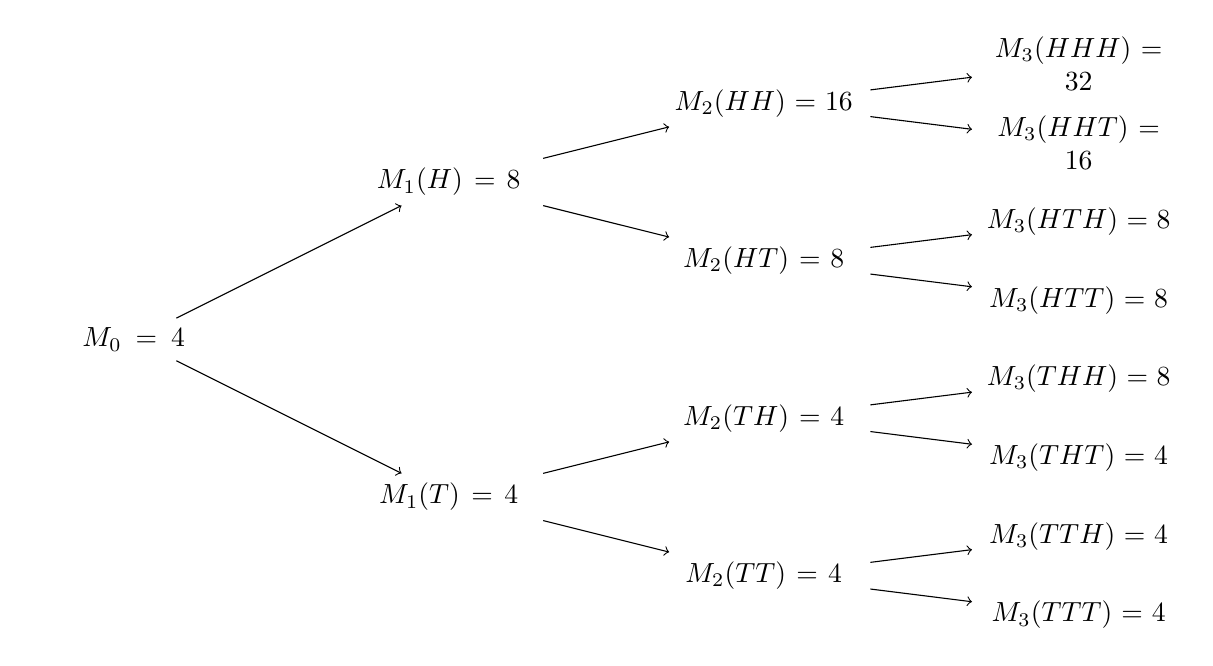
\begin{tikzpicture}[sloped]
  \node (a) at ( 0,0) [bag] {$M_0 = 4$};
  \node (b) at ( 4,-2) [bag] {$M_1(T) = 4$};
  \node (c) at ( 4,2) [bag] {$M_1(H) = 8$};
  \node (d) at ( 8,-3) [bag] {$M_2(TT) = 4$};
  \node (e) at ( 8,-1) [bag] {$M_2(TH) = 4$};
  \node (f) at ( 8,1) [bag] {$M_2(HT) = 8$};
  \node (g) at ( 8,3) [bag] {$M_2(HH) = 16$};
  \node (h) at ( 12,-3.5) [bag] {$M_3(TTT) = 4$};
  \node (i) at ( 12,-2.5) [bag] {$M_3(TTH) = 4$};
  \node (j) at ( 12,-1.5) [bag] {$M_3(THT) = 4$};
  \node (k) at ( 12,-0.5) [bag] {$M_3(THH) = 8$};
  \node (l) at ( 12,0.5) [bag] {$M_3(HTT) = 8$};
  \node (m) at ( 12,1.5) [bag] {$M_3(HTH) = 8$};
  \node (n) at ( 12,2.5) [bag] {$M_3(HHT) = 16$};
  \node (o) at ( 12,3.5) [bag] {$M_3(HHH) = 32$};
  \draw [->] (a) to node [below] {} (b);
  \draw [->] (a) to node [above] {} (c);
  \draw [->] (b) to node [below] {} (d);
  \draw [->] (b) to node [above] {} (e);
  \draw [->] (c) to node [below] {} (f);
  \draw [->] (c) to node [above] {} (g);
  \draw [->] (d) to node [below] {} (h);
  \draw [->] (d) to node [above] {} (i);
  \draw [->] (e) to node [below] {} (j);
  \draw [->] (e) to node [above] {} (k);
  \draw [->] (f) to node [below] {} (l);
  \draw [->] (f) to node [above] {} (m);
  \draw [->] (g) to node [above] {} (n);  
  \draw [->] (g) to node [above] {} (o);  
\end{tikzpicture}
\caption{$\max S_k$ process tree}
\end{figure}

\indent Consider the expectation $\E_2[M_3(\omega_3)](TH)$, that is, all realizations of the binomial tree after having the first two tosses $\omega_1 = T, \omega_2 = H$. We have
\begin{align*}
	\E_2[M_3(\omega_3)](TH) &= pM_3(THH) + qM_3(THT) \\
	&= \frac{2}{3}\cdot8 + \frac{1}{3}\cdot4 \\
	&= \frac{16}{3} + \frac{4}{3} = \frac{20}{3} \approx 6.6666...
\end{align*}

However we note that
\begin{equation*}
	\E_2[M_3(\omega_3)](TT) = 4
\end{equation*}

but
\begin{equation*}
	M_2(TH) = M_2(TT) = 4
\end{equation*}

Therefore, there cannot exist a function $g$ such that
\begin{align*}
	\frac{20}{3} &= \E_2[M_3(\omega_3)](TH) = g(M_2(TH)) = g(4) \\
	4 &= \E_2[M_3(\omega_3)](TT) = g(M_2(TT)) = g(4)
\end{align*}

since this would violate the vertical line test! Therefore $M_n$ is not Markovian in general.

\subsection{Multi-Dimensional Markov Processes}

\indent By adding one or more state variables (expanding the dimension of the process) we can often simplify a non-Markovian process to a Markovian one.

\begin{definition} Consider the binomial asset pricing model. Let $\{(X^1_n,...,X^K_n)\}^N_{n = 0}$ be a $K$-dimensional adapted process (a vector of $K$ one-dimensional adapted processes). If for every $n \in \{0,..., N - 1\}$ and for every function $f(x^1,...x^K)$ there exists a function $g(x^1,...,x^K)$, which may depend on $n$ and $f$, such that
\begin{equation*}
	\E_n \left[ f(X^1_{n + 1},...,X^K_{n + 1}) \right] = g(X^1_n,...,X^K_n)
\end{equation*}

then the process $\{(X^1_n,...,X^K_n)\}^N_{n = 0}$ is a \underline{$K$-dimensional Markov process}.
\end{definition}

\underline{Example}: In the binomial asset pricing model consider the maximum process $M_n = \max_{0 \leq k \leq N} \{S_k\}$ and the 2-dimensional adapted process $\{(S_n,M_n )\}^N_{n = 0}$. Show that this 2-dimensional process is Markovian. \\

\underline{Solution}: Define the random variable $Y$ such that
\begin{align*}
	Y = \frac{S_{n + 1}}{S_n}
	\begin{cases}
		u & \text{if } \omega_{n + 1} = H \\
		d & \text{if } \omega_{n + 1} = T
	\end{cases}
\end{align*}

then 
\begin{equation*}
	S_{n + 1} = YS_n
\end{equation*}

and
\begin{equation*}
	M_{n + 1} = \max \{M_n, S_{n + 1} \} = \max \{M_n, YS_n\}
\end{equation*}

\indent It is clear that $(M_n, S_n)$ depends only on the first $n$ coin tosses and so it is an adapted process. Note that $Y$ does not depend on the first $n$ coin tosses (i.e. it is independent of the first $n$ tosses) and only depends on the $n + 1^{\text{th}}$ coin toss. Since $(S_n, M_n)$ depend only on the first $n$ coin tosses we have by the Independence Lemma
\begin{align*}
	\E_n [ f(S_{n + 1}, M_{n + 1} ) ] &= \E_n [ f(YS_n, \max \{M_n, YS_n\}  ] \\
	&= \E_n [ f^*(S_n, M_n, Y) ] \\
	&= g(S_n, M_n)
\end{align*}

where
\begin{align*}
	g(s,m) &= \E [ f^*(s,m,Y) ] \\
	&= \E [ f(Ys, \max \{m, Ys \}) ] \\
	&= pf(us, \max \{m, us\}) + qf(ds, \max \{m, ds\})
\end{align*}

for arbitrary function $f$. That is, we have found a $g$ satisfying the definition. Hence $(S_n,M_n)$ is a 2-dimensional Markov process. \\

\indent Suppose that we have some Markov process $\{X_n\}^N_{n = 0}$ and $0 \leq n \leq N - 2$. Then the Markov property implies that for every function $h$ there exists some $f$ such that
\begin{equation*}
	\E_{n + 1}[h(X_{n + 2})] = f(X_{n + 1})
\end{equation*}

\indent Taking the conditional expectation of both sides with respect to the information available at time $n$ 
\begin{align*}
	\E_n \left[ \E_{n + 1}[h(X_{n + 2})] \right] &= \E_n \left[ f(X_{n + 1}) \right] \\
	\E_n [h(X_{n + 2})] &= \E_n[f(X_{n + 1})] \quad \text{(by the tower property)}
\end{align*}

However, by the one-step Markov property of $X$ there exists a $g$ such that
\begin{equation*}
	\E_n[f(X_{n + 1})] = g(X_n) 
\end{equation*}

Hence
\begin{equation*}
	\E_n[h(X_{n + 2})] = \E_n[f(X_{n + 1})] = g(X_n)
\end{equation*}

\indent Repeating this argument we can show that if $\{X_n\}^N_{n = 0}$ is a Markov process, for $0 \leq n \leq m \leq N$, and any function $h$, there exists a function $g$ (which may depend on $f$, $n$, and $m$) such that
\begin{equation*}
	\E_n[h(X_m)] = g(X_n)
\end{equation*}

\indent Similarly, the above {\bf multi-step Markov property} holds for a $K$-dimensional vector valued Markov process. That is, if $\{(X^1_n,...,X^K_n)\}_{n = 1}^N$ is Markovian then, whenever $0 \leq n \leq m \leq N$, for arbitrary function $h$ there exists another function $g$ satisfying
\begin{equation*}
	\E_n[h(X^1_m,...,X^K_m)] = g(X^1_m,...,X^K_m)
\end{equation*}

\indent In the binomial model suppose that $\{X_n\}^N_{n = 0}$ is Markovian and the payoff of a derivative security at time $N$ is $V_N$ which is some function $\nu_N$ of  $X_N$, that is
\begin{equation*}
	V_N(\omega_1\cdots\omega_N) = \nu_N(X_N(\omega_1\cdots\omega_N)) \quad \forall~ \omega_1\cdots\omega_N \in \Omega
\end{equation*}

The risk neutral pricing formula gives us
\begin{equation*}
	V_n = \tilde{\E}_n \left[ \frac{V_N}{(1 + r)^{N - n}} \right]
\end{equation*}

However, the multi-step Markov property gives
\begin{equation*}
	\tilde{\E}_n \left[ \frac{V_N}{(1 + r)^{N - n}} \right] = \tilde{\E}_n \left[ \frac{ \nu_N(X_N) }{(1 + r)^{N - n}} \right] = \nu_n(X_n)
\end{equation*}

for some function $\nu_N$. Therefore, the price of the derivative security at time $n$ is a function of $X_n$
\begin{equation*}
	V_n = \nu_n(X_n)
\end{equation*}

\indent This fact can lead to potentially less computationally intensive algorithm for calculating $V_n$ since the argument of $V_N$ is the sequence $\omega_1\cdots\omega_N$ whereas the argument of $\nu_N$ is simply some real number.










\end{document}
